\documentclass[10pt, conference, compsocconf]{IEEEtran}

\usepackage{amsfonts}
\usepackage{amssymb,amsmath}
\usepackage{hyperref}
\usepackage{algorithm}
\usepackage{algpseudocode}
\usepackage{graphicx}
\usepackage[skip=2pt,font=footnotesize]{caption}


% http://blog.mikael.johanssons.org/archive/2012/03/biblatex-%E2%80%94-why-havent-i-used-this-earlier/
\usepackage{biblatex}
%\usepackage[citestyle=authoryear]{biblatex}
\addbibresource{ref.bib}
\renewcommand*{\nameyeardelim}{\addspace}
\renewcommand*{\revsdnamedelim}{\addspace}

% correct bad hyphenation here
\hyphenation{op-tical net-works semi-conduc-tor}

% path for images
\graphicspath{ {../figs/generated/} }

\makeatletter
\renewcommand{\ALG@beginalgorithmic}{\footnotesize}
\renewcommand{\alglinenumber}{\footnotesize}
\setlength{\belowcaptionskip}{0pt plus 0pt minus 0pt}
\setlength{\abovecaptionskip}{0pt plus 0pt minus 0pt}
\makeatother

\begin{document}
\renewcommand*{\nameyeardelim}{\addspace}
\renewcommand*{\revsdnamedelim}{\addspace}
%
% paper title
% can use linebreaks \\ within to get better formatting as desired
\title{A Recommender Framework for Portfolio Selection to Reduce
Fraud in Electricity Distribution Using Integer Programming and Heuristic Techniques}



% author names and affiliations
% use a multiple column layout for up to two different
% affiliations

\author{\IEEEauthorblockN{Diego Luchi \IEEEauthorrefmark{1}, 
F\'abio Fabris \IEEEauthorrefmark{2}, 
Marcos Daniel Valad\~ao Baroni,
Alexandre Rodrigues,
Fl\'avio Miguel Varej\~ao}
\IEEEauthorblockA{N\'ucleo de Infer\^encia em Algoritmos (NINFA) - Departamento de Inform\'atica\\
Universidade Federal do Esp\'irito Santo\\
Vit\'oria, Esp\'irito Santo, Brasil\\
}
\IEEEauthorblockA{\IEEEauthorrefmark{1}
E-mail: dluchi@ninfa.inf.ufes.br
}
\IEEEauthorblockA{\IEEEauthorrefmark{2}
E-mail: ffabris@ninfa.inf.ufes.br
}
}



% make the title area
\maketitle


\begin{abstract}
Electricity fraud corresponds to a major source of loss in Electricity
Distribution Companies in developing countries. To attenuate this,
companies have at their disposal several loss reduction actions. These actions
must be performed to reach a given electricity loss reduction goal, established
by the regulatory agency. If this goal is not reached, the profit margin
of the company is reduced.
This work defines a formal model for the action allocation task 
and proposes an exact mathematic programming method for solving small instances of
the problem and two heuristic methods for larger ones. We compare
the techniques considering solution quality.

\end{abstract}

\begin{IEEEkeywords}
Optimization; Metaheuristics; Knapsack;
\end{IEEEkeywords}


% For peer review papers, you can put extra information on the cover
% page as needed:
% \ifCLASSOPTIONpeerreview
% \begin{center} \bfseries EDICS Category: 3-BBND \end{center}
% \fi
%
% For peerreview papers, this IEEEtran command inserts a page break and
% creates the second title. It will be ignored for other modes.
\IEEEpeerreviewmaketitle



The multidimensional knapsack problem (MKP) is a strongly NP-hard combinatorial
optimization problem which can be viewed as a resource allocation problem and
defined as follows:

\begin{align*}
  \text{maximize} & \sum_{j=1}^n p_j x_j \\
  \text{subject to} & \sum_{j=1}^n w_{ij} x_j \leqslant c_i \quad i \in \{1, \ldots, m\}\\
   & x_j \in \{0, 1\}, \quad j \in \{1, \ldots, n\}.
\end{align*}

% Define the MKP
The problem can be interpreted as a set of $n$ items with profits $p_j$
and a set of $m$ resources with capacities $c_i$.
Each item $j$ consumes an amount $w_{ij}$ from each resource $i$, if selected.
The objective is to select a subset of items with maximum total profit,
not exceeding the defined resource capacities.
The decision variable $x_j$ indicates if $j$-th item is selected.

The multidimensional knapsack problem can be applied on budget planning 
scenarios, subset project selections, cutting stock problems, task scheduling,
allocation of processors and databases in distributed computer programs.
The problem is a generalization of the well-known knapsack problem (KP) in which
$m = 1$.

The MKP is a NP-hard problem significantly harder to solve in practice than the KP.
Despite the existence of a fully polynomial approximation scheme (FPAS) for the KP,
finding a FPAS for the MKP is NP-hard for $m \geqslant 2$~\cite{magazine1984note}.
Due its simple definition but challenging difficulty the MKP is often used to
to verify the efficiency of novel metaheuristics.

Its well known that the hardness of a NP-hard problem grows exponentially over
its size.
Thereupon, a suitable approach for tackling those problems is to reduce their size
through some variable fixing procedure.
Despite not guaranteeing optimality of the solution, an efficient variable
fixing procedure may provide near optimal solutions through a small computational effort.

%A metaheuristic is a set of concepts that can be used to define heuristic methods
%that can be applied to a wide set of different problems.
%In other words, a metaheuristic can be seen as a general algorithmic framework which can be applied to
%different optimization problems with relatively few modifications to make them adapted to a specific problem.”

The SCE is a metaheuristic, proposed by Duan in \cite{duan1992effective},
which combines the ideas of a controlled random search with the concepts
of competitive evolution and shuffling.
The SCE algorithm has been successfully used to solve several problems
like flow shop scheduling~\cite{zhao2014shuffled} and project management~\cite{elbeltagi2007modified}.

In this paper we address the development of a hybrid heuristic for the MKP.
The size of the problem instance is first reduced through a variable fixing
procedure that uses a known concept among knapsack problems called \emph{core}.
The reduced problem is then efficiently solved by a SCE algorithm.

The reminder of the paper is organized as follows:
Section~\ref{sec:core} defines the core concept for the MKP and its application
for the problem reduction.
Section~\ref{sec:sce} presents the shuffled complex evolution algorithm
and proposes its application on the MKP.
Section~\ref{sec:exp} comprises several computational experiments over well-known
instances from literature.
In section~\ref{sec:conc} we make our concluding remarks about the developed
methods and the experimental results.



To apply optimization algorithms in our problem we first need to define it formally. Lets assume
that we must maximize the \textit{net present value} (the present investment return considering 
inflation) for a reduction plan of $M$ years, given:

\begin{itemize}
    \item a yearly budget for a set of $L$ resources $o_{il}$, $1 \le i \le M$, $1 \le l \le L$;
    
    \item a fraud reduction goal $g_i$, $1 \le i \le M$ that represents the
    amount of electricity loss that must be reduced;

    \item an \textit{internal rate of return} $r$, that represents the yearly depreciation of the investment
    (constant for all investments and years). 

\end{itemize}

We also assume that there are several actions to choose from a portfolio of actions of size $N$.
Each action $j$, $1 \le j \le N$, contained in the portfolio has several parameters: 
\begin{itemize}
    \item the electricity value $v_j$, that represents the value of the unit of electricity for each action $j$ in portfolio,
    i.e., the value of each Kilowatt of electricity;
    \item $m_j$, the maximum number of times that action $j$ may be performed, we
    shall refer to it as \textit{the market} of the action;
    \item $u_{j,i}$ the maximum number of times that action $j$ may be performed in the $i$-th year;
    \item $c_{j,l}$, the $l$-th cost associated to each execution of action $j$;
    \item $e_{j,k}$, the amount of lost electricity that the action $j$ will reduce after 
    $k$ years it was executed, when taken once;
    \item a set $D_j \subset \mathbb{N^*}$ that represents which actions must be performed prior action $j$.
    For each action $j$ the action $D_{j,d}$ ($1 \le d \le |D_j|$) must be executed a number of times defined by
    \item the parameter $Q_{j,d} \in \mathbb{R^+}$.
\end{itemize}

Our objective is to find a set of values for variables $x_{j,i}$, $\forall i,j$, $x_{j,i} \in \mathbb{N} $, 
the number of times that the action $j$ will be performed in the $i$-th year. We wish to choose a combination
of values that maximizes the net present value and is under the fraud reduction goal for all years. 

The constraints of the problem are the yearly budget restriction,
\begin{equation}
    \sum_{j=1}^{N} x_{j, i} \cdot c_{j,l} \le o_{i,l} \, \forall i, l,
	\label{eq:budget}
\end{equation}
the market restriction,
\begin{equation}
     \sum_{i=1}^{M} x_{j, i} \le m_j \, \forall j,
	\label{eq:market}
\end{equation}
the maximum number of times the action $x_{j, i}$ may be performed in $i$-th year,
\begin{equation}
     x_{j, i} \le u_{j, i} \, \forall j, i,
	\label{eq:maxacts}
\end{equation}
the goal restriction,
\begin{equation}
    \label{eq:goal}
    \sum_{j=1}^{N} \sum_{k=1}^{M}R_{i,j,k}(\bar{x}) \leq g_i \, \forall i, \\
\end{equation}
$R_{i,j,k}$ being the fraud reduction in the $k$-th year by the action $j$ taken on $i$-th year, defined as
\begin{equation}
    \label{eq:rec}
    R_{i,j,k}(\bar{x}) = x_{j, i} \cdot e_{j, k - i + 1} \, \forall k \geq i,
\end{equation}
and the dependency restriction for all actions and for all years,
\begin{equation}
    \label{eq:dependency}
    \forall j,k \quad \sum_{i=1}^{k} x_{d, i} \ge x_{j, d} \cdot Q_{j, d} \, \forall d \in D_j.
\end{equation}

To introduce the objective function we must define some auxiliary concepts:
The yearly total cost, $C_i$,
\begin{equation}
\label{eq:cost}
C_{i}(\bar{x}) =  \sum_{j=1}^{N} \sum_{l=1}^{L} x_{j, i} \cdot c_{j,l} \, \forall i,
\end{equation}
the gained profit in $i$-th year, due to elimination of the fraud, $V_i$,
\begin{equation}
    V_{i}(\bar{x}) = \sum_{j=1}^{N} \sum_{k=1}^{M} R_{k, j, i}(\bar{x}) \cdot v_j \, \forall i,
\end{equation}
by definition $V_i - C_i$ is the total cash flow in $i$-th year. 

Finally, we may define the objective function as:
\begin{equation}
    \label{eq:objective}
    max(O(\bar{x})) = max\left(\sum_{i=1}^{M} \frac{V_i(\bar{x}) - C_i(\bar{x})}{(1+r)^i}\right).
\end{equation}

The objective function represents the net present value, that is,
the sum of the yearly cash flows, $V_i - C_i$, adjusted by the internal rate of return for all years.

\subsection{Realistic Version}

To adapt the previously defined problem to the current state of our local EDCO, we simplify it in several  ways:

\begin{itemize}
%terminar de editar
\item We consider that the yearly budgets are insufficient to surpass the goal for any given year;
%because this is usually the case in real world scenarios. %This consideration
%renders the equation~\ref{eq:objective} imprecise. 

\item We consider all actions on portfolio have an positive cash flow;

\item We ignore the dependencies among actions, that is, the set $D_j$ is empty
for all actions; %This is necessary to simplify the analysis we perform in this work.

\item We assume that both the vectors that define the costs of the $j$-th  action $c_j$
and the $i$-th budget $o_i$ have size 1;%, that is, actions use resources of only
%one kind.

\item We assume that the electricity  value $v_j$ is constant for all actions;

\item We assume that the value of $\sum_{i=0}^{N} u_{j,i} \leq m_j, \forall j$.
%Meaning that there is no yearly limit to the amount of times actions may be
%performed.

\end{itemize}

The simplifications may be altered accordingly to the current
state of the distributer. Other companies may eliminate or consider other restrictions,
and as far as we know, the model is general enough to model for the
majority of possible scenarios.

%\todo[inline]{Terminar seção.}






\section{Related Work} 
\label{sec:relat}

The exact formulation of the problem has shown to be quite particular and
no work addressing a similar problem was found in literature.
If the depreciation of the investments is not considered ($r=0$),
the problem may  be viewed as a \textit{Partially-Ordered Multidimensional
Multiple Knapsack Problem} (POMMKP). Which is, as far as we know, a
novel version of the classical Knapsack Problem.

Additionally, If we consider just the cost $c_{j,l}$ of each action (weight), the
reduction of lost electricity  $e_{j,k}$ of each action (profit) and the yearly budget (capacity)
on a single year situation ($M=1$) the problem could be classified as a simple
\textit{Knapsack Problem}~\cite{pisinger1995}.
If we now add the dependency restriction, the problem could be considered
a \textit{Partially-Ordered Knapsack Problem}~\cite{pok2002}.
If we consider multiple years ($M > 1$) instead of the dependency restriction, it would characterize
a \textit{Multiple Knapsack Problem}, with each year with its own capacity.
Considering multiple resources ($M=1, L > 1$) and no dependency, the problem can be formulated as a
\textit{Multidimensional Knapsack Problem}.

All the problems mentioned above are hard to solve optimally, these problems are known 
as $\mathcal{NP}$-hard problems and are no know polynomial time algorithms to solve, unless $\mathcal{P} = \mathcal{NP}$.
For the classical knapsack problem there is a FPTAS (\textit{Fully Polynomial Time Approximation Scheme}),
while for the others variants mentioned above are hard to aproximate and there are only PTAS 
(\textit{Polynomial Time Approximation Scheme}) to solve them with a certain degree of 
approximation of the optimal solution, ~\cite{pok2002, puchinger2006core, dawande2000approximation}. 

The POMMKP can be considered as a generalization of the above mentioned problems,
thus we may conclude that POMMKP is at least as difficult as any of them.
Since our problem is a generalization of the POMMKP, it is as difficult as the POMMKP.
For this reason there is no algorithm that solves our problem in polynomial time (considering
$\mathcal{P} \ne \mathcal{NP}$).
Given the difficulty of approximating the optimal solution of this problem through exact algorithms, heuristics methods are necessary 
for solving larger instances of the problem.

% \section{Coupled-Knapsack Approach}
\label{sec:knap}



To solve our allocation problem we have developed three methodologies: 1) an exact algorithm
using integer programming, 2) a heuristic Gradient Ascent algorithm using the LP-relaxed version of the integer
programming model as a starting solution (GALP) and 3) a Tabu Search
algorithm that also uses the LP solution as a starting point (TSLP). In the following subsections we present each approach and comment on their particularities.
%The implementation of all methos is available at 

%To solve our allocation problem we have developed three methodologies: an exact approach
%and two heuristic algorithms.
%The exact approach considered the realistic version of the MIP formulation, previously defined on Section~\ref{sec:defi}.
%The first heuristic algorithm applies a gradient ascent method on an initial solution from a LP-relaxed model of the MIP formulation.
%
%The second heuristic algorithm takes this same initial 
%
%As duas baordagens heuristicas sao inicializadas com uma solucao inicial 
%As outras duas abordagens heuristicas sao inicializadas com a solucao otima truncated do LP-relaxation of the original formulation.
%
%using integer programming and two heuristic algorithms using the LP-relaxed version of MIP
%with an a-posteriori heuristic allocation scheme.
%algorithm. In the following subsections we present each approach and comment on their particularities.

\subsection{Exact Mathematical Programming Approach}
The exact approach considers the realistic version of the 
MIP formulation, previously defined in Section~\ref{sec:defi}.
To solve this formulation, we have used a branch-and-bound method~\cite{lawler1966branch}
included in the GLPK solver \cite{GLPK}.

\subsection{Gradient Ascent using the LP solution (GALP)}
%However this method is known to get stuck in local minima.
We use a simple heuristic approach, namely Gradient Ascent (GA), using
the truncated solution of the relaxed version of the linear problem (considering $x_{j,i} \in [0,u_{j,i}]$) as a initial search point.
Since the relaxed version of the linear problem is easily solvable by the simplex 
algorithm ~\cite{dantzig1955generalized} and the Gradient Ascent algorithm has 
fast convergence characteristics, this approach is very efficient, 
converging in less than 10 iterations in most of our test instances. 
However because it is a greedy heuristic, it has the flaw of getting stuck in local minima,
because it never accepts a solution if it is worse than the current one.
Algorithm \ref{alg:ga} depicts the procedure.

We have compared the solution quality randomly starting the $GA$ algorithm in different locations of the
search space and found that in our experiments it never found a better solution
than using the truncated Linear Problem solution as a start.

%\begin{figure}
\begin{algorithm}[H]
\begin{algorithmic}[1]
\Function{Gradient Ascent}{Initial solution $S_{ini}$}
\State $S_{best} \gets S_{ini}$
\State $HasImproved \gets True$
\While{$HasImproved$}
    \State $HasImproved \gets False$
    \For{\label{alg:neigh}Each $Neig$ in $Neighborhood(V_{best})$}
        \If{$Evaluate(Neig) > Evaluate(S_{ini})$}
            \State $S_{best} \gets Neig$
            \State $HasImproved \gets True$
        \EndIf
    \EndFor
\EndWhile
\State \Return $S_{best}$
\EndFunction
\end{algorithmic}
\caption{Gradient Ascent Algorithm}
\label{alg:ga}
\end{algorithm}
%\end{figure}

Line \ref{alg:neigh} of the algorithm uses the function $Neighborhood(Solution)$, that
returns a set containing all possible solutions generated from $Solution$ by adding a
single action to the current solution.


\subsection{Tabu Search using the LP solution (TSLP)}

The second applied technique was the Tabu Search algorithm ~\cite{glover1997tabu}, again using the Linear Programming solution as the initial candidate solution. In~\cite{puchinger2010}, the authors claim that Tabu Search initialized with LP solution is the best known method to solve Multidimensional Knapsack Problem. We expect that the Tabu Search algorithm to be more prone to scape
local minima, since it can accept solutions worst than the current one. 
The pseudocode is depicted in the algorithm~\ref{alg:ts} ~\cite{brownlee2011clever}.

We have also compared the solution quality if we randomly start the $TS$ algorithm in the
search space and found that in our experiments it never found a better solution
than using the truncated Linear Problem solution as a start.

%\begin{figure}
\begin{algorithm}[H]
\begin{algorithmic}[1]
\Function{Tabu Search}{Initial solution $S_{ini}$}
\State $S \gets S_{ini}$
\State $S_{best} \gets S$
\State $TabuList \gets \emptyset$
\While{$StoppingCondition$}
    \State $CandList \gets \emptyset$
    \For{\label{alg:tabuneig}Each $S_{cand}$ in $TabuNeighborhood(S)$}
        \If{$featureDiff(S_{cand},S) \notin TabuList$}
            \State $CandList \gets CandList + S_{cand}$
        \EndIf
    \EndFor
    \State $S \gets BestCand(CandList)$
    \If{$Fitness(S) > Fitness(S_{best})$}
        \State $TabuList \gets TabuList + featureDiff(S, S_{best})$
        \State $S_{best} \gets S$
        \While{$size(TabuList) > maxSize$}
            \State $RemoveOldest(TabuList)$
        \EndWhile
    \EndIf
\EndWhile
\State \Return $S_{best}$
\EndFunction
\end{algorithmic}
\caption{Tabu Search Algorithm}
\label{alg:ts}
\end{algorithm}
%\end{figure}

The for loop on Line \ref{alg:tabuneig} uses the function $TabuNeighborhood(Solution)$,
that returns a neighborhood of  solutions generated from $Solution$.
In our case, we chose to return in this list the same neighborhood of GALP
concatenated with a randomly generated set of size $n_{tabu}$ that differ from the base solution
by at most three actions. For instance, if $Solution = \{10, 12, 30, 10\}$, a possible return of
$TabuNeighborhood(Solution)$ could be $\{\{12, 11, 30, 10\},\{10,12,29,10\},\{9,11,30,10\}\}$.

%We opted to use the actual solution of the problem as a tabu element instead of a movement.
%Albeit this is not the standard approach, we have found it to be more effective, converging
%faster and yielding statistical equivalent results in comparison to the standard approach
%in our problem.





\subsection{Experimental Setup}
\subsubsection{Computational Environment}
All experiments were run in Intel Core i5-2310 CPU @ 2.90GHz machines
with 8GB of RAM memory running Linux Mint 13 64 bits.  To facilitate the job distribution we have used the HTCondor framework.

\subsubsection{Parameters}
The GALP algorithm has no settable parameters, the TSLP algorithm on the other hand,
has 3 parameters: the number of iterations of the Tabu Search algorithm (10000),
the size of the tabu list (1000) and the number of random neighbors per iteration
($n_{tabu}$ = 500).
The parameters were set up by empirically experimenting several different combinations.

\subsubsection{Implementation}
To solve the integer programming problems we have used the GLPK LP/MIP solver \cite{GLPK},
version 4.43. We have implemented the heuristics using the Java programming language and
executed/compiled the codes using the Java(TM) SE Runtime Environment (build 1.7.0\_10-b18).
All implementations are available at \url{http://ninfa.inf.ufes.br/ICTAI2013/impl.zip}. 

\subsection{Instance Generator}
To create the instances for our analysis we have implemented a random instance generator.
We have tried to mimic the characteristics of real-world actions supplied by the local EDCO.
Algorithm~\ref{alg:gen} defines the pseudocode of the random instance generator.

\begin{figure}
\begin{algorithm}[H]
\begin{algorithmic}[1]
\Function{Generator}{Correlation factor $\alpha$, Number of years $M$, Number of actions $N$}
\State \label{line:gen1} $BudgetMean \gets Random_{\textit{Uniform}}(700,800)$
\State $BudgetVariance \gets Random_{\textit{Uniform}}(10,20)$
\For{$i=1 \to M$}
  \State $o_{i1} \gets Random_{\textit{Gauss}}(BudgetMean,$ $BudgetVariance)$
\EndFor \label{line:gen2}
\For{$j=1 \to N$}\label{line:gen3}
  \State $c_{j1} \gets \label{line:min} Min(Min(o), Random_{\textit{Uniform}}(1,100))$
\EndFor
\For{$j=1 \to N$}
  \State \label{line:market} $ m_j = 2 Sum(o) / (M \cdot c_{j1})$
\EndFor \label{line:gen4}

\For{$j=1 \to N$} \label{line:W1}
  \For{$i=1 \to M$}
    \State $W_{ji} \gets Random_{\textit{Uniform}}(0,1)$
  \EndFor
  \State $W_{j} \gets ReverSort(W_{j})$
\EndFor

\For{$j=1 \to N$}
  \State $s \gets 0$
  \For{$i=1 \to M$}
    \State $s \gets s + W_{ji}$
  \EndFor
  \For{$i=1 \to M$}
    \State $W_{ji} \gets W_{ji}/s$
  \EndFor
\EndFor  \label{line:W2}

\For{$i=1 \to M$} \label{line:e1}
  \For{$j=1 \to N$}
      \State \label{line:en} $e_{j,k} \gets Max(0, Abs((1-\alpha) \cdot c_{j1} \cdot W_{ji} \, +$
      \State $\qquad \quad \, Random_{\textit{Uniform}}(-100,100) \cdot \alpha))$
  \EndFor
\EndFor \label{line:e2}
\EndFunction
\end{algorithmic}
\caption{Random instance generator}
\label{alg:gen}
\end{algorithm}
\end{figure}

Lines \ref{line:gen1} to \ref{line:gen2} present the generation of the yearly budgets from a Gaussian
distribution (function $GaussRandom(mean, variance)$) that in turn has its variance and mean draw 
from a uniform distribution of fixed parameters (function $URandom(Lower\,bound,\,Upper\,bound)$).
The parameters were inspired by real-world actions, given by the local EDCO.

Lines \ref{line:gen3} to \ref{line:gen4} generate the cost and market of each action, the cost comes from
an uniform random distribution with fixed parameters. Note that in line \ref{line:min} we
use the $Min$ function to guarantee that the action may performed at least one time. Line \ref{line:market}
defines the market of each action as a function of the total budget over all years ($Sum(o)$) and the
cost of the action. That is, the cheapest the action the larger the market.

Lines \ref{line:W1} to \ref{line:W2} are used to build the reverse-ordered normalized weight matrix that is used to 
build the recuperation over the years. After line \ref{line:W2}, the $j$-th line of matrix $W$ will contain
a vector of values that add up to 1 and are reversely ordered, e.g., a possible $W$ matrix for 3 years and 4 actions
could be:
\[ W = \left( \begin{array}{ccc}
0.7 & 0.2 & 0.1 \\
0.8 & 0.1 & 0.1 \\
0.6 & 0.2 & 0.2 \\
1.0 & 0.0 & 0.0 \end{array} \right).\] 

Finally from lines \ref{line:e1} to \ref{line:e2} the electricity recuperation values are defined for each action
and each year. In line \ref{line:en} we may see that the use of matrix $W$ guarantees that the electricity recuperation has a decreasing tendency
over the years. In this line we also present the use of the correlation parameter $\alpha \in [0,1]$.
The closest $\alpha$ is to one, the weaker is the correlation.

The generator was implemented in the Python programming language and its implementation 
and random instances are available at \url{http://ninfa.inf.ufes.br/ICTAI2013/gen.zip}.

\subsection{Time Analysis}

\subsubsection{The Impact of Correlation}                      
It has been demonstrated the classical  Knapsack Problem is pseudo-polynomial
in the size of the input \cite{garey1978} and it is a established
fact that a weak correlation among weight and value greatly reduces the difficulty of the instances \cite{david2005}.
Literature on the knapsack problem states that the difficult problems are the ones that exhibit 
a strong correlation between the value of the item and its weight.

To test if this phenomena also happens in our problem, we have tested the values $[0.0, 0.1, 1.0]$ for $\alpha$,
the parameter that controls the correlation of the value of the action in respect to its cost, 
in a number of problem sizes. When $\alpha$ is 0,
there is a strong correlation between the cost of the action and its electricity return, that is,
the more expensive the action, the more effective it is. When $\alpha$ is 1 there is no correlation
between the value of the actions and its effectiveness. When $\alpha$ is 0.1, there is a weak correlation between cost and value.
The $\alpha$ values of 0.0, 0.1 and 1.0 are equivalent to the following classes of problems defined by \cite{david2005} (respectively): 
\textit{subset sum instances, weakly correlated instances and uncorrelated instances.}

To measure running times we have generated instances for each considered $\alpha$, varying both the amount of years and actions
in the interval $[5,15]$. For each triple defined by the value of $\alpha$, the number of years and actions,
we have generated 10 instances and measured their running time to find the exact solution. 
We have observed that the variance of the running times to solve these 10 instances was too large
for the mean to be significative, so we have adopted a alternative strategy to compare problem sizes
and $\alpha$:
we assume that running times of more than one hour are prohibitive for our application, since
EDCO's usually test several portfolios to make their investment decision. So we consider that
these instances failed to find the solution in practical times.

Figures~\ref{fig:time1} to~\ref{fig:time3} display the amount of instances that successfully executed in less than one hour,
given a value of $\alpha$. For each cell of the figure the exact algorithm was run 10 times using random instances of the problem.
The closer to black, the greater the amount of successful runs. 
From the figures it is clear that the bigger the problem the more likely it is that it will take more than one hour to execute, 
since cells closer to $(15,15)$ tend to be closer to white.
Also, it may be observed that the more
correlated the cost is with the profit (the smaller the $\alpha$),
the harder the problems seems to be, as predicted by the literature.

%\begin{subfigure}[b]{0.3\textwidth}
%  \includegraphics[width=\textwidth]{mouse}
%  \caption{A mouse}
%  \label{fig:mouse}
%\end{subfigure}

\begin{figure}
  \begin{subfigure}
    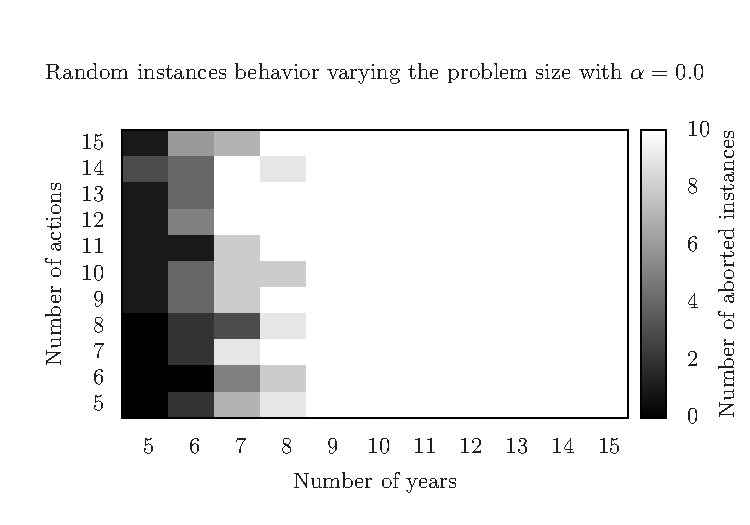
\includegraphics[scale=0.73, trim=0.75cm 0cm 0 2cm, clip=true]{imgs/very_hard.pdf}
    \caption{Strong correlation between cost and profit.}
    \label{fig:time1}
  \end{subfigure}
  \begin{subfigure}
    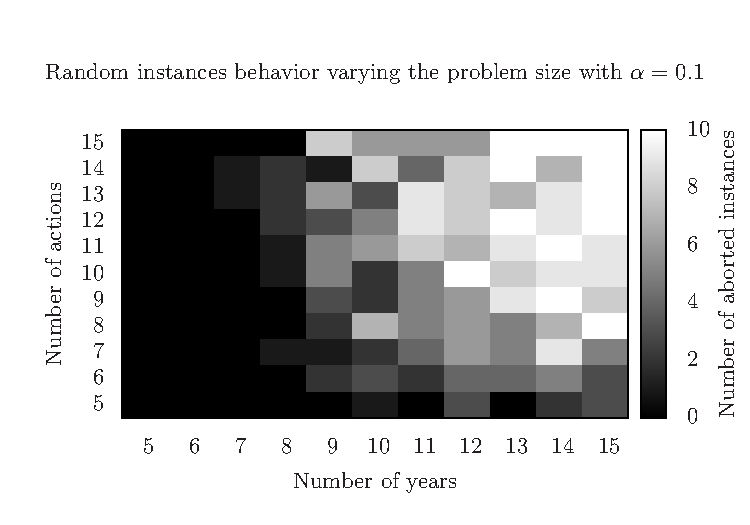
\includegraphics[scale=0.73, trim=0.75cm 0cm 0 2cm, clip=true]{imgs/hard.pdf}
    \caption{Weak correlation between cost and profit. \\ $\,$ }
    \label{fig:time2}
  \end{subfigure}
\end{figure}

\begin{subfigure}
  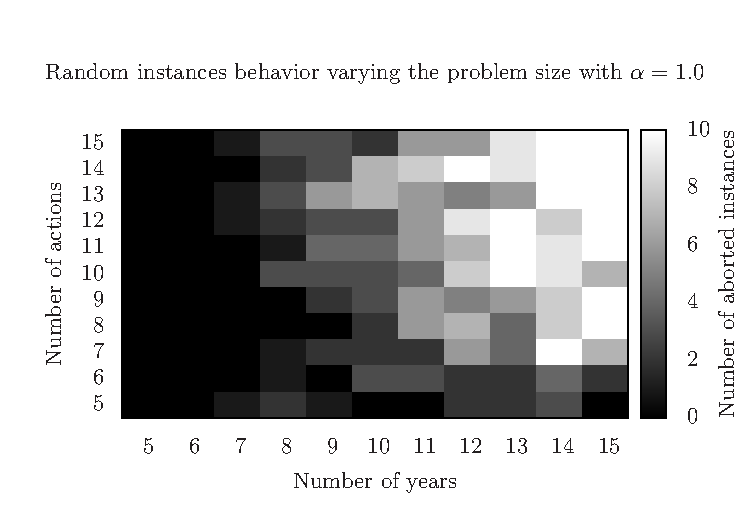
\includegraphics[scale=0.73, trim=0.75cm 0cm 0 2cm, clip=true]{imgs/easy.pdf}
  \caption{No correlation between cost and profit.}
  \label{fig:time3}
\end{subfigure}


\subsection{Solution Analysis - Easy Instances}

In this subsection we compare the solution quality of the implemented heuristics
in the set of easy instances, there is, the instances in which the exact algorithm
found the optimal solution in less than one hour. We have also limited the running time
of the heuristics in one hour.

Figures~\ref{fig:mh1_1} to \ref{fig:mh2_3} display the average ratio between the optimal solution (when available) 
and the solution found by the heuristics. 
Small relative ratios are darker than large differences.
A ratio of 1 means that the heuristic has found a solution with the same quality
than the exact algorithm.
When no solution was found by the exact approach in less than one hour for 
a tripe $(\alpha, years, actions)$, we display the value ``$na$'' in
the corresponding cell.

Figures~\ref{fig:mh1_1} to \ref{fig:mh2_3} show that all heuristics managed
to find very close solutions to the exact (less than 1\% difference).
Also, the paler aspect of the TSLP figures (specially when $\alpha=0.0$) suggests that
it managed to beat the GALP algorithm considering solution quality.
In fact, considering only these easier problem sizes, the paired Wilcoxon signed-rank test \cite{japkowicz2011evaluating} rejects the null hypothesis
that the algorithms are the same with a $p$-value of less than $10^{-11}$.

\begin{figure}
\centering
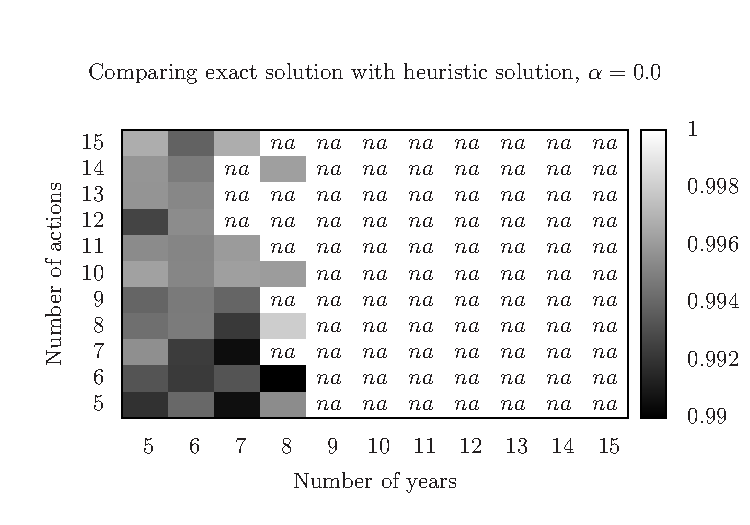
\includegraphics[scale=0.73, trim=0.75cm 0cm 0 2cm, clip=true]{imgs/comp_very_hard.pdf}
\caption{Comparison between the optimal solution (when available) 
and the solution by the GALP for $\alpha=0.0$.}
\label{fig:mh1_1}
\end{figure}

\begin{figure}
\centering
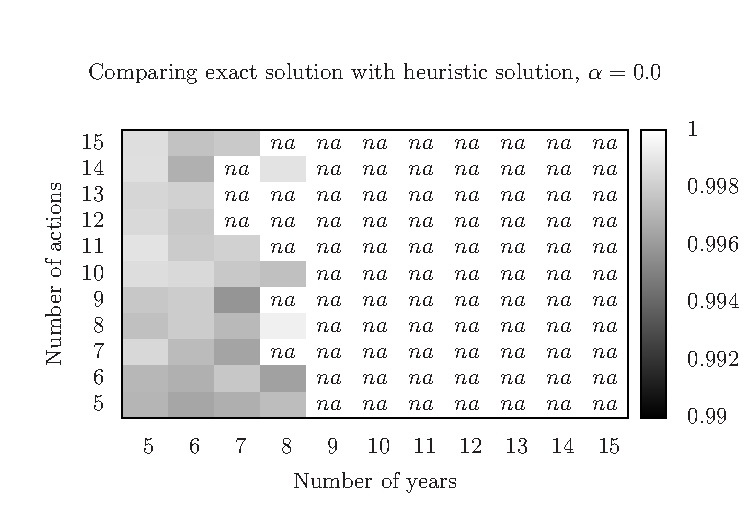
\includegraphics[scale=0.73, trim=0.75cm 0cm 0 2cm, clip=true]{imgs/comp_very_hard_ts.pdf}
\caption{Comparison between the optimal solution (when available) 
and the solution by the TSLP for $\alpha=0.0$.}
\label{fig:mh2_1}
\end{figure} 

\begin{figure}
\centering
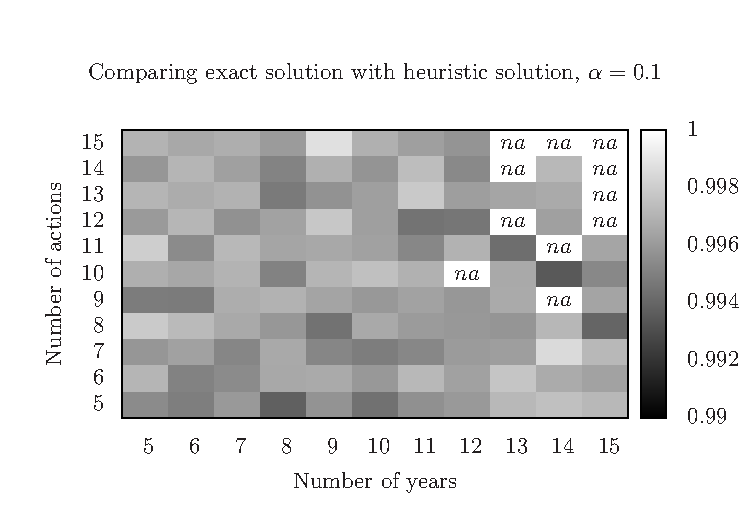
\includegraphics[scale=0.73, trim=0.75cm 0cm 0 2cm, clip=true]{imgs/comp_hard.pdf}
\caption{Comparison between the optimal solution (when available) 
and the solution by the GALP for $\alpha=0.1$.}
\label{fig:mh1_2}
\end{figure}

\begin{figure}
\centering
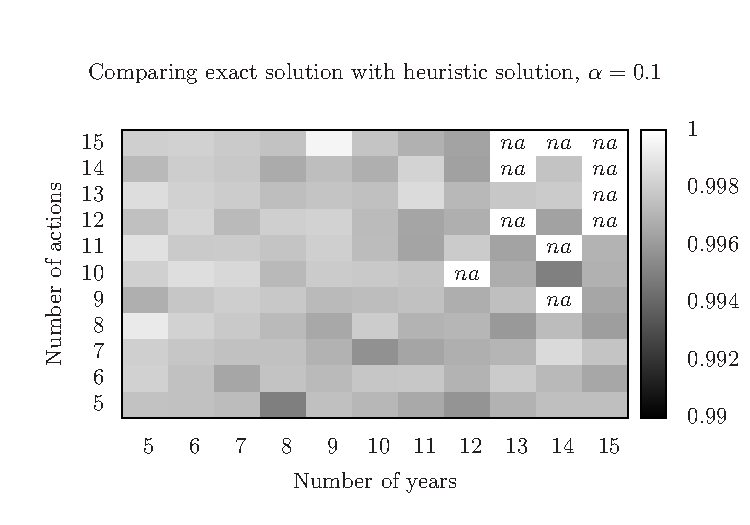
\includegraphics[scale=0.73, trim=0.75cm 0cm 0 2cm, clip=true]{imgs/comp_hard_ts.pdf}
\caption{Comparison between the optimal solution (when available) 
and the solution by the TSLP for $\alpha=0.1$.}
\label{fig:mh2_2}
\end{figure}
 
\begin{figure}
\centering
%\vspace{1mm}
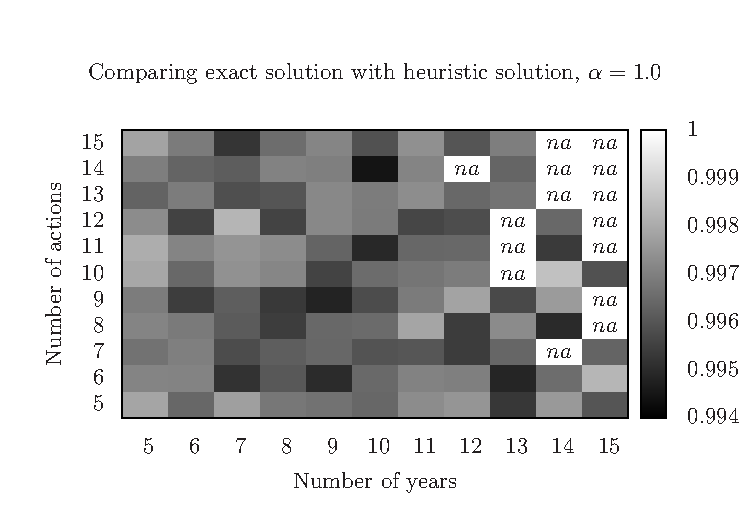
\includegraphics[scale=0.73, trim=0.75cm 0cm 0 2cm, clip=true]{imgs/comp_easy.pdf}
\caption{Comparison between the optimal solution (when available) 
and the solution by the GALP for $\alpha=1.0$.}
\label{fig:mh1_3}
\end{figure}

\begin{figure}
\centering
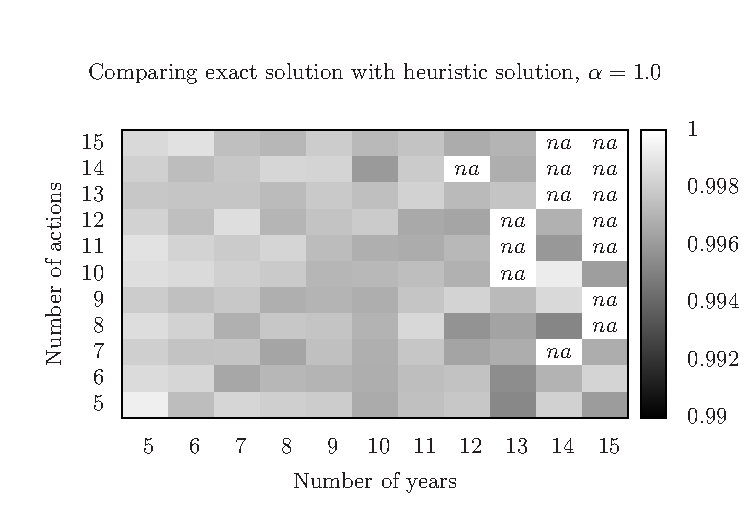
\includegraphics[scale=0.73, trim=0.75cm 0cm 0 2cm, clip=true]{imgs/comp_easy_ts.pdf}
\caption{Comparison between the optimal solution (when available) 
and the solution by the TSLP for $\alpha=1.0$.}
\label{fig:mh2_3}
\end{figure}


\subsection{Solution Analysis - All Instances}

In this subsection we compare the behavior of the metaheuristics in respect to one another
considering all instances. We cannot compare the results with the optimal solution since they are unknown for the harder instances.

Figures~\ref{fig:comp_1} to \ref{fig:comp_3} display the relative distance between the two proposed 
heuristics considering the solution quality for the three studied correlation values.
Each cell contains the mean ratio between the quality of the GAPL and TSLP algorithms,
here the mean is meaningful because the values of the ratio have a reasonable variance.

From the scale of the figures (varying between 1 and 0.993 at most) it is clear
that both algorithms achieved very similar results, however the TSLP algorithm
managed to outperform the GAPL, in average, in every cell of the figures (no value is greater than 1).
However GALP did manage to outperform the TSLP algorithm in some instances of the problem,
so we perform the paired Wilcoxon signed-rank to confirm that the TSLP is indeed superior
to the GALP algorithm. And again we may reject that null hypothesis that the algorithm
are equal with a $p$-value of less than $10^{-11}$.

\begin{figure}
\centering
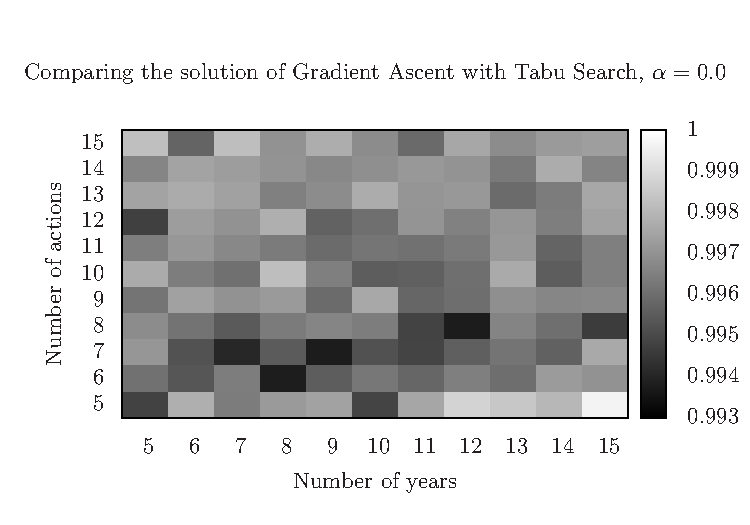
\includegraphics[scale=0.73, trim=0.75cm 0cm 0 2cm, clip=true]{imgs/comp_very_hard_sg_ts.pdf}
\caption{Relative distance between the two proposed heuristics for $\alpha=0.0$.}
\label{fig:comp_1}
\end{figure}


\begin{figure}
\centering
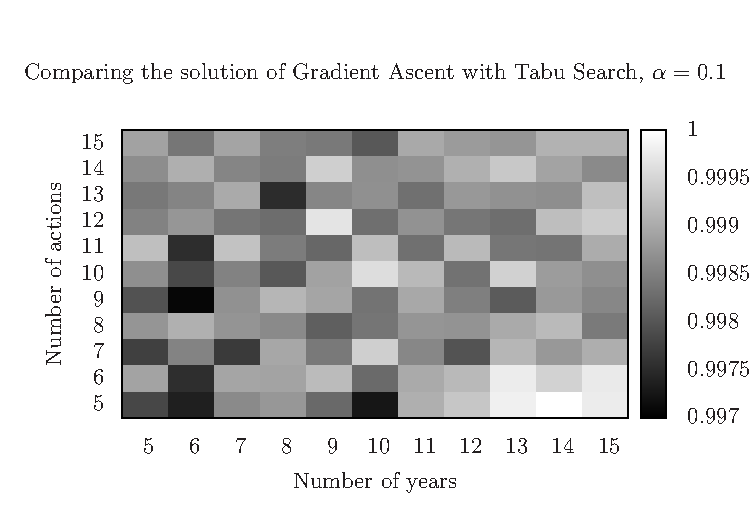
\includegraphics[scale=0.73, trim=0.75cm 0cm 0 2cm, clip=true]{imgs/comp_hard_sg_ts.pdf}
\caption{Relative distance between the two proposed heuristics for $\alpha=0.1$.}
\label{fig:comp_2}
\end{figure}

\begin{figure}
\centering
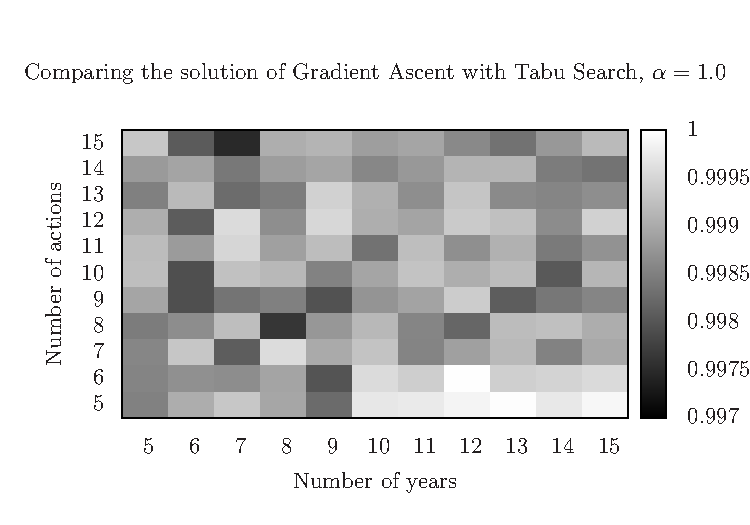
\includegraphics[scale=0.73, trim=0.75cm 0cm 0 2cm, clip=true]{imgs/comp_easy_sg_ts.pdf}
\caption{Relative distance between the two proposed heuristics for $\alpha=1.0$.}
\label{fig:comp_3}
\end{figure}

Figures~\ref{fig:lpgavsmip} and \ref{fig:lptsvsmip} display the histogram of
the ratio of the solution found by the heuristic algorithms and the optimal solution.
From the histograms we can conclude that TSLP has a better behavior than GALP,
showing a smaller variance and larger ratio mean.

Although the time limit was set to one hour, the TSLP had a maximum running time of less than one minute, with an average time of 20 seconds, and GALP had a negligible running time for all instances.

\begin{figure}
\centering
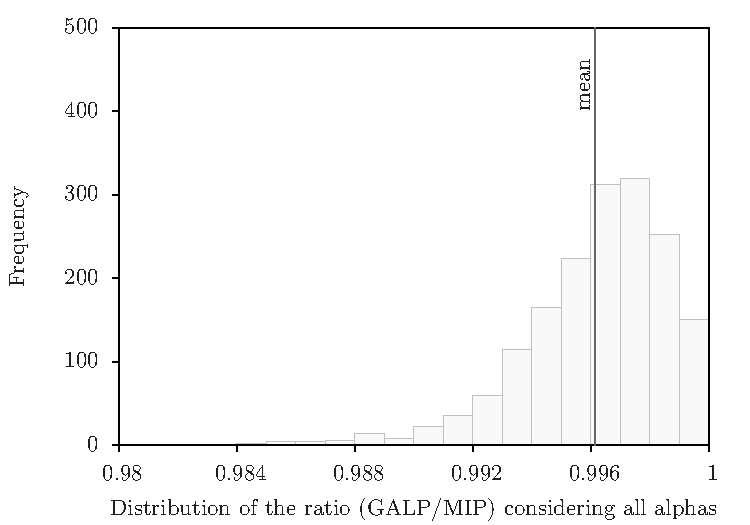
\includegraphics[scale=0.7, trim=1cm 0 0 0]{imgs/lpgavsmip.pdf}
\caption{Histogram of the ratio of the solution found by the GALP heuristic and the optimal solution.}
\label{fig:lpgavsmip}
\end{figure}

\begin{figure}
\centering
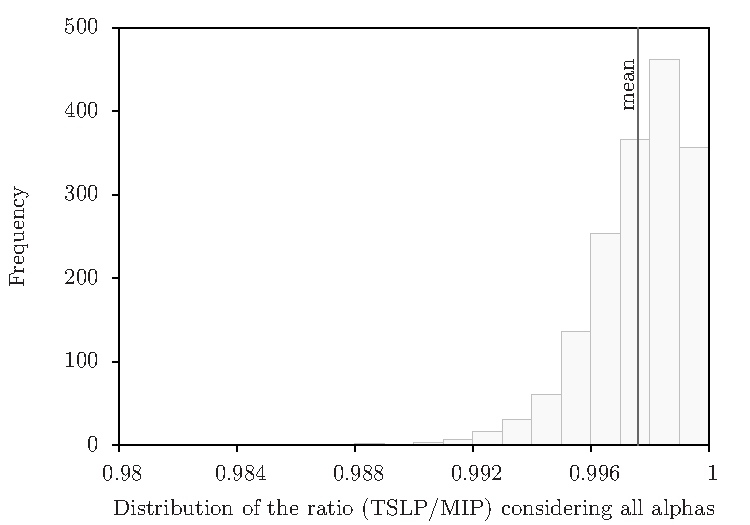
\includegraphics[scale=0.7, trim=1cm 0 0 0]{imgs/lptsvsmip.pdf}
\caption{Histogram of the ratio of the solution found by the TSLP heuristic and the optimal solution.}
\label{fig:lptsvsmip}
\end{figure}

% From the figures it is clear that the TSLP algorithm is superior



\section{Conclusion and Future Work}
\label{sec:con}

This works presents a modeling of a relevant problem to Electricity Distribution Companies in developing countries.
The modeling yields a challenging optimization problem. We propose a exact technique to solve easier instances
of the problem and two heuristics to tackle the more difficult instances.

We conclude that our incarnation  of the classical Knapsack is sensible to the correlation between weight and cost, as
predicted by the literature on the problem.

We have tested two heuristic algorithm, namely Tabu Searh using the Linear Problem solution as an initial search point
(TSLP) and Gradient Ascent using the Linear Problem solution as an initial search point (GALP), both achieving good solutions and
execution times. In particular, the TSLP algorithm was statically better than the GALP algorithm
in our test instances, with bigger running times.

Future work includes the investigation an algorithm for the complete version of the problem and
a deeper study of what makes some instances take more time than others despite 
having the same amount of years, actions and $\alpha$ and being randomly generated
in a similar way.

\vspace{1cm}


\printbibliography

% that's all folks
\end{document}


